\documentclass[a4paper]{article}
% Shared preamble for the English probability and statistics documents.
% Based on the original course preamble. Compile with pdfLaTeX.
\usepackage[top=1.5cm,bottom=2cm,left=2cm,right=2cm]{geometry}
\usepackage[T1]{fontenc}
\usepackage{lmodern}
\usepackage[utf8]{inputenc}
\usepackage[english]{babel}

\usepackage{amsmath}
\usepackage{amssymb}
\usepackage{amsthm}
\usepackage{mathrsfs}
\usepackage{mathtools}
\usepackage{etoolbox}
\usepackage{tikz}
\usetikzlibrary{shapes.multipart,arrows.meta}
\usepackage{xcolor}
\usepackage{enumerate}
\usepackage[shortlabels]{enumitem}
\usepackage{hyperref}
\usepackage{version}
\usepackage{bbold}
\usepackage{fontawesome5}
\usepackage{fancyhdr}
\lfoot{}
\usepackage{natbib}
\usepackage{graphicx}
\usepackage{pdfpages}
\usepackage{authblk}
    
\usepackage{blindtext}
\usepackage{multicol}
\usepackage{collcell}
\usepackage{wrapfig}
\usepackage{blkarray}
\usepackage{cancel}
\usepackage{appendix}
\usepackage{float}
\makeatletter
\input{tex/assets/slashbox.sty}
\makeatother
\hypersetup{unicode,colorlinks,citecolor=red,filecolor=black,
  linkcolor=red,urlcolor=cyan}
\setlength{\columnsep}{1cm}
\pagenumbering{gobble}

\def\numtext#1{%
  \ifcase#1\or one\or two\or three\or four\or five\or six\or seven\or eight\or nine\or ten\or
  eleven\or twelve\or thirteen\or fourteen\or fifteen\or sixteen\or seventeen\or eighteen\or nineteen\or twenty\or Lots\fi}

\newcommand{\Byte}[1]{%
  \def\nodecontents{}%
  \foreach[count=\l] \k in {#1} {\xappto{\nodecontents}{\noexpand\nodepart{\numtext{\l}}\k}}%
  \node[rectangle split,rectangle split parts=8,rectangle split horizontal,draw] at (2,2){\nodecontents};}

\newcommand{\D}{{\mathrm{d}}}
\newcommand{\cE}{{\mathcal{E}}}
\newcommand{\cG}{{\mathcal{G}}}
\newcommand{\cX}{{\mathcal{X}}}
\newcommand{\cY}{{\mathcal{Y}}}
\newcommand{\cB}{{\mathcal{B}}}
\newcommand{\cF}{{\mathcal{F}}}
\newcommand{\cO}{{\mathcal{O}}}
\newcommand{\cS}{{\mathcal{S}}}
\newcommand{\cT}{{\mathcal{T}}}
\newcommand{\given}{\, \big| \,}
\newcommand{\cL}{{\mathscr{L}}}
\newcommand{\cD}{{\mathcal{D}}}
\newcommand{\cA}{{\mathscr{A}}}
\newcommand{\cP}{{\mathscr{P}}}
\newcommand{\cR}{{\mathscr{R}}}
\newcommand{\A}{{\mathcal A}}
\newcommand{\one}{\mathbb{1}}
\newcommand{\mathbbm}[1]{\mathbb{#1}}

\providecommand{\C}{}
\renewcommand{\C}{\mathbb C}
\newcommand{\R}{\mathbb R}
\newcommand{\Q}{\mathbb Q}
\newcommand{\N}{\mathbb N}
\newcommand{\T}{\mathbb T}
\newcommand{\F}{\mathbb F}
\renewcommand{\P}{\mathbb P}
\newcommand{\Z}{\mathbb Z}
\newcommand{\E}{\mathbb {E}}
\newcommand{\Pbb}[1]{\P\left( #1\right)}
\newcommand{\Ebb}[1]{\E\left[ #1\right]}

\newcommand{\lb}{\left (}
\newcommand{\rb}{\right )}
\newcommand{\lbb}{\left [}
\newcommand{\rbb}{\right ]}
\newcommand{\labs}{\left |}
\newcommand{\rabs}{\right |}
\newcommand{\lbrb}[1]{\lb #1 \rb}
\newcommand{\lbbrbb}[1]{\lbb#1\rbb}
\newcommand{\labsrabs}[1]{\labs#1\rabs}
\newcommand{\lbbrb}[1]{\lbb#1\rb}
\newcommand{\lbrbb}[1]{\lb#1\rbb}
\newcommand{\langlerangle}[1]{\langle#1\rangle}
\newcommand{\lbcurly}{\{}
\newcommand{\rbcurly}{\}}
\newcommand{\curly}[1]{\lbcurly#1\rbcurly}
\newcommand{\abs}{\labsrabs}
\newcommand{\ind}[1]{1_{#1}}
\newcommand{\indep}{\perp \!\!\! \perp}
\renewcommand{\d}{\, \mathrm{d}}

\newtheorem{theorem}{Theorem}
\newtheorem{problemCnt}{Lemma}
\theoremstyle{definition}
\newtheorem{problem}[problemCnt]{Problem}
\newtheorem{problembook}[problemCnt]{\faBook \,  Problem}
\newtheorem{problempencil}[problemCnt]{\faPencil* \,  Problem}
\newtheorem{problemstar}[problemCnt]{\faStar\,  Problem}
\newtheorem{problemstarpencil}[problemCnt]{\faStar \, \faPencil* \,   Problem}
\newtheorem{probleminteresting}[problemCnt]{\faSmile[regular] \,   Problem}
\newtheorem{solution}{Solution}

\newcommand{\fwcell}[1]{\makebox[\arraystretch\normalbaselineskip]{$#1$}}
\newenvironment{enumeratei}{\begin{enumerate}[(i)]}{\end{enumerate}}
\newenvironment{enumeratea}{\begin{enumerate}[(a)]}{\end{enumerate}}
\newenvironment{enumeraten}{\begin{enumerate}[\upshape 1.]}{\end{enumerate}}

% Compatibility helpers needed by a few files in the combined archive.
\AtBeginDocument{\noindent{\footnotesize English translation prepared with ChatGPT (OpenAI, GPT-6), 26 October 2026, for translation of the Bulgarian text into English and LaTeX formatting.
The Bulgarian originals remain the reference; translation may contain errors.}\par\smallskip}
\newcommand{\MissingGraphic}[1]{%
  \begin{center}\fbox{\parbox{0.82\linewidth}{\centering Missing source image: \texttt{#1}}}\end{center}}



\setlength{\emergencystretch}{3em}
\allowdisplaybreaks
\begin{document}
\noindent Software Engineering \hfill Exam, 06.02.2025: solutions
\par\smallskip\hrule\smallskip\noindent

\textit{English transcription of the handwritten solutions. Calculations and unfinished answers are retained as written in the original.}

\section*{1. Waiting for three heads}
\begin{enumerate}
\item
\[
\P(Y=n)=\binom{n-1}{2}p^3(1-p)^{n-3}.
\]
There are two heads among the first $n-1$ tosses, and the $n$th toss is heads.
Write $Y=X_1+X_2+X_3$, where the $X_i$ are iid $\operatorname{Ge}(p)$; thus $\boxed{\E Y=3/p}$.
\item
\[
\P(Y\leq2k)=\sum_{i=3}^{2k}\binom{i-1}{2}p^3(1-p)^{i-3}.
\]
This can also be evaluated explicitly, but there is no need. As $k\to\infty$, $\P(Y\leq2k)\to1$.
For any random variable $X$, $\P(X\leq k)\to1$ as $k\to\infty$.
\end{enumerate}

\section*{2. The two boxes}
\begin{enumerate}
\item Intuitively, $5.5$ looks like the right answer. It should not matter whether we choose a random subset and then a random element of it, or directly choose a random element of the initial set. A formal argument can be given in several ways, for example by calculating that each number is selected with probability $1/10$. This is almost identical to the first question of Problem 1.6 in Test 1, 01.12.2024.
\item There are five pairs summing to 11: $(1,10),(2,9),\dots$.
The probability of choosing any one pair is $1/4$, and of not choosing it is $3/4$.
Thus
\[
\P(\text{none of the pairs is selected})=(\tfrac34)^5,
\qquad
\text{answer: }1-(\tfrac34)^5.
\]
\item If $K$ is the number of slips transferred from A, then $N$ is geometric conditionally on $K$.
$K$ is random, so an unconditional statement with a random parameter is not meaningful.
The notes give the following conditional-expectation calculation:
\[
\E[N|K]=\frac1K
\quad\Longrightarrow\quad
\E N=\E[\E[N|K]]=\E[1/K],
\]
\[
\E N=\sum_{n=1}^{10}\frac1n\P(K=n)
=\frac1{10}(1+2+\dots+10).
\]
The idea is the same as Problem 2 from Test 1 in Probability and Statistics, 2021.
\end{enumerate}

\section*{3. Densities}
The first three parts are standard. Recall
\[
\E[\operatorname{Exp}(1)]=\int_0^\infty xe^{-x}\,dx=1,\qquad
D[\operatorname{Exp}(1)]=1,\qquad \int_0^\infty x^2e^{-x}\,dx=2.
\]
\begin{enumerate}
\item Normalization gives
\[
k\int_0^\infty xe^{-x}\,dx=1\quad\Longrightarrow\quad \boxed{k=1}.
\]
For the triangular joint-density region,
\begin{align*}
1&=c\int_0^1\int_0^{1-x}(x+y)\,dy\,dx\\
&=c\int_0^1\left((1-x)x+\frac{(1-x)^2}{2}\right)\,dx\\
&=\frac c2\int_0^1(-x^2+1)\,dx=\frac c2(-\tfrac13+1)=\frac c3,
\end{align*}
so $\boxed{c=3}$. Furthermore,
\[
\E X=\int_0^\infty x^2e^{-x}\,dx=2.
\]
By symmetry, $\E Y=\E Z$, and
\begin{align*}
\E Y&=c\int_0^1\int_0^{1-x}y(x+y)\,dy\,dx\\
&=c\int_0^1\left(x\frac{(1-x)^2}{2}+\frac{(1-x)^3}{3}\right)\,dx\\
&=\frac c6\int_0^1(3x-6x^2+3x^3+2-6x+6x^2-2x^3)\,dx\\
&=\frac c6\int_0^1(x^3-3x+2)\,dx
=\frac c6(\tfrac14-\tfrac32+2)=\frac12\cdot\frac34=\frac38.
\end{align*}
\item
\[
\P(X>2)=\int_2^\infty xe^{-x}\,dx,\qquad
\int xe^{-x}\,dx=-\int x\,de^{-x}=-xe^{-x}-\int e^{-x}\,dx=-xe^{-x}-e^{-x}.
\]
The handwritten numerical conclusion is $\P(X>2)=0+e^{-1}+e^{-1}=2e^{-1}$.
Also,
\begin{align*}
\P(Y>\tfrac12)&=c\int_0^{1/2}\int_{1/2}^{1-x}(x+y)\,dy\,dx\\
&=c\int_0^{1/2}\left[x(\tfrac12-x)+\frac{(1-x)^2-\frac14}{2}\right]\,dx\\
&=c\int_0^{1/2}\frac18(4x-8x^2+4-8x+4x^2-1)\,dx\\
&=\frac38\int_0^{1/2}(-4x^2-4x+3)\,dx
=\frac38(-4\cdot\tfrac1{24}-4\cdot\tfrac18+\tfrac32)
=\frac38\cdot\frac56=\frac5{16}.
\end{align*}
\item
\[
\E[YZ]=c\int_0^1\int_0^{1-x}xy(x+y)\,dy\,dx=\dots=\frac1{10}.
\]
Hence
\[
\operatorname{Cov}(Y,Z)=\frac1{10}-\frac9{64}
=-\frac{13}{320}\neq0,
\]
so $Y,Z$ are not independent. For $\E[Z|Y=3/8]$, use the conditional density. Since $X$ and $Y$ are independent, $\E[X|Y]=\E X$.
The conditional expectation $\E[Z|Y]$ is the random variable $g(Y)$, where $g(y)=\E[Z|Y=y]$ is obtained as in the first case.
\item To find the density of $YZ$, put $V=YZ$, $W=Y$. The inverse is $Y=W$, $Z=V/W$, and
\[
|J|=\left|\begin{matrix}0&1\\1/w&*\end{matrix}\right|=\frac1w.
\]
Thus
\[
f_{V,W}(v,w)=f_{Y,Z}(w,v/w)\frac1w
=c\left(w+\frac vw\right)\one_{\{w,v>0,\ w+v/w<1\}}\frac1w.
\]
Since $w>0$, $w+v/w<1$ is equivalent to $w^2-w+v<0$. The roots are
\[
w_{1,2}=\frac{1\pm\sqrt{1-4v}}2.
\]
The region lies below $v=w-w^2$, so $0<v<1/4$ and
\[
\frac{1-\sqrt{1-4v}}2<w<\frac{1+\sqrt{1-4v}}2.
\]
Consequently,
\begin{align*}
f_V(v)&=3\int_{(1-\sqrt{1-4v})/2}^{(1+\sqrt{1-4v})/2}
\left(1+\frac v{w^2}\right)\,dw\\
&=3\left[\sqrt{1-4v}
-\frac{2v}{1+\sqrt{1-4v}}+\frac{2v}{1-\sqrt{1-4v}}\right]\\
&=3\left[\sqrt{1-4v}
-\frac{2v(1-\sqrt{1-4v})}{4v}
+\frac{2v(1+\sqrt{1-4v})}{4v}\right]\\
&=6\sqrt{1-4v},\qquad 0<v<1/4.
\end{align*}
\end{enumerate}
\begin{center}
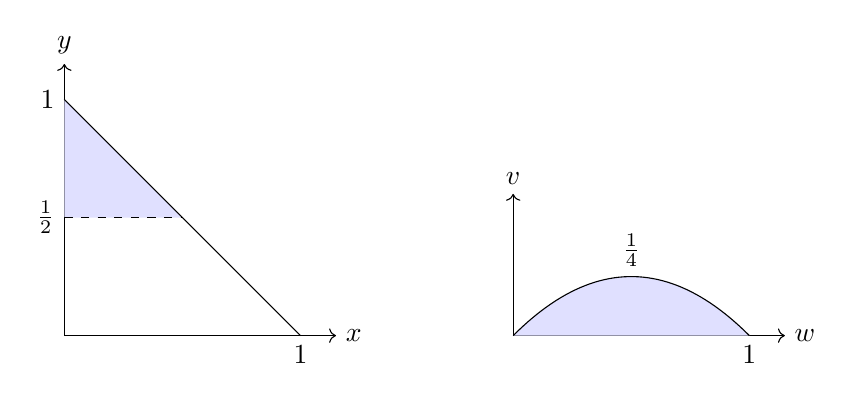
\begin{tikzpicture}[scale=3]
\draw[->](0,0)--(1.15,0)node[right]{$x$};
\draw[->](0,0)--(0,1.15)node[above]{$y$};
\fill[blue!12](0,0.5)--(0,1)--(0.5,0.5)--cycle;
\draw(0,1)--(1,0);
\draw[dashed](0,0.5)--(0.5,0.5);
\node[left]at(0,0.5){$\frac12$};\node[left]at(0,1){$1$};\node[below]at(1,0){$1$};
\begin{scope}[xshift=1.9cm]
\draw[->](0,0)--(1.15,0)node[right]{$w$};
\draw[->](0,0)--(0,0.6)node[above]{$v$};
\fill[blue!12]plot[domain=0:1,samples=50](\x,{\x-\x*\x})--cycle;
\draw plot[domain=0:1,samples=50](\x,{\x-\x*\x});
\node[above]at(0.5,0.25){$\frac14$};\node[below]at(1,0){$1$};
\end{scope}
\end{tikzpicture}
\end{center}

\section*{4. Random permutations}
\begin{enumerate}
\item Choose the other $k-1$ elements in the cycle containing 1, arrange them, and permute the remaining elements:
\[
\P(1\text{ is in a cycle of length }k)
=\frac{\binom{n-1}{k-1}(k-1)!(n-k)!}{n!}
=\frac{(n-1)!}{n!}=\frac1n.
\]
\item Observe
\[
\sum_{i=1}^n\one_{\{i\text{ is in a cycle of length }k\}}
=k\,(\text{number of cycles of length }k).
\]
Taking expectations and using part 1 gives $n/n=k\,\E[\text{number of cycles of length }k]$. By linearity,
\[
\E[c(\sigma)]=\E\left[\sum_{k=1}^n\text{number of cycles of length }k\right]
=1+\frac12+\dots+\frac1n.
\]
For fixed points,
\[
\P(\sigma(1)=1)=\P(1\text{ is fixed})=\P(i\text{ is fixed})
=\E[\one_{\{i\text{ is fixed}\}}]=\frac1n.
\]
Thus $\E[F(\sigma)]=\E[\sum_{i=1}^n\one_{\{i\text{ is fixed}\}}]=n/n=1$.
\item This is Problem 21 in the file on Moodle.
\item Yes; use an appropriate CLT for weakly dependent random variables. One can show that $\E[c(\sigma)]$ and $D[c(\sigma)]$ are asymptotic to $\log n$, and consider how to represent $c(\sigma)$ as a sum of random variables.
\end{enumerate}
\end{document}
